\documentclass[12pt]{article}
\usepackage[english]{babel}
\usepackage{natbib}
\usepackage{url}
%\usepackage[utf8x]{inputenc}
\usepackage{amsmath}
\usepackage{graphicx}
\graphicspath{{images/}}
\usepackage{parskip}
\usepackage{float}
\usepackage{fancyhdr}
\usepackage[nottoc,numbib]{tocbibind}
%\usepackage{vmargin}


\title{P4: Mohr's Circle Lab Report}								% Title
\author{Jack Tyler}								% Author
\date{\today}											% Date

\makeatletter
\let\thetitle\@title
\let\theauthor\@author
\let\thedate\@date
\makeatother

\pagestyle{fancy}
\fancyhf{}
\rhead{\theauthor}
\lhead{\thetitle}
\cfoot{\thepage}

\begin{document}

%%%%%%%%%%%%%%%%%%%%%%%%%%%%%%%%%%%%%%%%%%%%%%%%%%%%%%%%%%%%%%%%%%%%%%%%%%%%%%%%%%%%%%%%%

\begin{titlepage}
	\centering
    \vspace*{0.5 cm}
    %
\includegraphics[scale = 0.75]{UCT.jpg}\\[1.0 cm]	% University Logo
    \textsc{\LARGE University of Southampton}\\[2.0 cm]	% University Name
	\textsc{\Large FEEG1002}\\[0.5 cm]				% Course Code
	\textsc{\large Mechanics, Structures and Materials}\\[0.5 cm]				% Course Name
	\rule{\linewidth}{0.2 mm} \\[0.4 cm]
	{ \huge \bfseries \thetitle}\\
	\rule{\linewidth}{0.2 mm} \\[1.5 cm]
	
	\begin{minipage}{0.4\textwidth}
		\begin{flushleft} \large
			\emph{Author:}\\
			\theauthor
			\end{flushleft}
			\end{minipage}~
			\begin{minipage}{0.4\textwidth}
			\begin{flushright} \large
			\emph{Student Number:} \\
			27513556									% Your Student Number
		\end{flushright}
	\end{minipage}\\[2 cm]
	
	{\large \thedate}\\[2 cm]
 
	\vfill
	
\end{titlepage}
\tableofcontents
\newpage
%%%%%%%%%%%%%%%%%%%%%%%%%%%%%%
%%%%%%%%%%%%%%%%%%%%%%%%%%%%%%
\section{Summary}
%No Text Here
%%%%%%%%%%%%%%%%%%%%%%%%%%%%%%%
\textit{Concise, covering all aspects of the report.}

%%%%%%%%%%%%%%%%%%%%%%%%%%%%%%%
\section{Introduction}
Mohr’s circle is a graphical method to determine the effect of a coordinate rotation on a tensor quantity. In the engineering sciences it is applied to analyse the effect of a coordinate rotation on \textit{stress, strain, second moment of area} and \textit{moment of inertia}. In this experiment, Mohr's circle was applied to readings of strain gauges to determine principal stresses in multiple frames of reference, as well as Poisson's ratio for each reference frame. The results found from the Mohr's circle were cross-checked against predictions from Beam Theory. \\

In wider Engineering applications, Mohr's circle is used to determine stresses in rotated coordinate systems from a material body assumed to be continuum. This proves useful in experimental testing for rating materials for expected lifetime loading, such as components for buildings, transport systems and mass-market devices. Typically used in conjunction with strain gauges, as here, the Circle can provide graphical representations of two- and three-dimensional stresses, as well as failure criteria. It is particularly useful for supplementing computer-based simulations of component loading for verification of acceptable loading characteristics, and can be used in tandem with Lame's stress ellipsoid and Cauchy's stress quadric.

%%%%%%%%%%%%%%%%%%%%%%%%%%%%%%%%%%%%%%%%%

\section{Objectives}

The prime objectives of this experiment were as follows:

\begin{enumerate}
	\item Be able to apply Mohr's circle to effectively determine the state of strain at a point on a beam and its material properties.
	\item Validate relationships set out by Beam Theory as part of Part I Statics, allowing for understandings of the ideas behind them.
	\item Gain experience in the usage of strain gauges for projects in Part II onwards.
\end{enumerate}

%-----------------------------------

\section{Experiment}
\subsection{Apparatus}
\subsubsection{Apparatus Layout}
An aluminium alloy beam is clamped at one end within a rig containing a cam whose full-range rotation leads to a repeatable tip deflection of $\Delta$ = 12.5 mm, as shown in Figure \ref{exp1}. The beam has dimensions as follows: breadth b = 25.4 mm, depth d = 6.35 mm and length (to the cam) L = 254 mm. Three strain gauges are mounted on the upper surface at 94 mm from the clamped end; these gauges are mounted at 15$^{\circ}$, 45$^{\circ}$, and 75$^{\circ}$ with respect to the longitudinal x-axis of the beam, as shown in Figure \ref{exp2}. Each of these gauges can be selected using a switchboard to be one arm of a Wheatstone bridge arrangement, with a dummy strain gauge providing temperature compensation. \footnote{This was later replaced with a fixed resistor incapable of providing temperature fluctuation adjustment. The effect of this is outlined in the portion of the report associated with the critique of the experiment.}
\begin{figure}[ht]
	\graphicspath{{C:/Users/Jack/Pictures/}}
	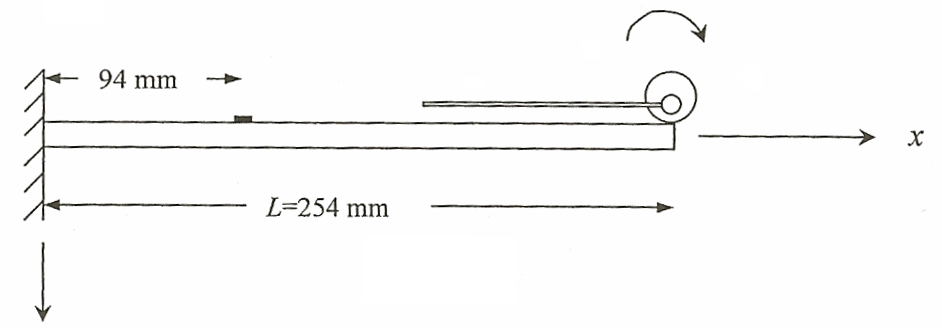
\includegraphics[width=\linewidth]{experiment1}
	\centering
	\caption{\label{exp1} Schematic of the Clamped Beam and Cam}
\end{figure}
%---------------------------------------
\begin{figure}[H]
	\graphicspath{{C:/Users/Jack/Pictures/}}
	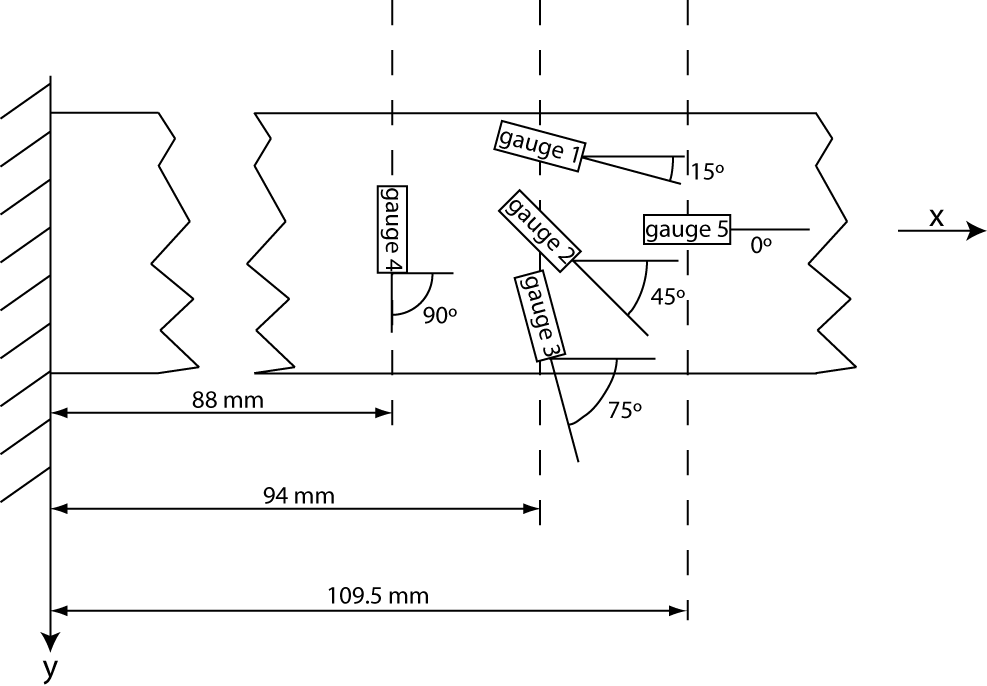
\includegraphics[width=\linewidth]{experiment2}
	\caption{\label{exp2} Schematic of Strain Gauges 1-5 as mounted on top of the beam}
\end{figure}
\newpage

\subsubsection{Apparatus Theory: Strain Gauges}
A strain gauge consists of thin metal wire arranged into a grid, as shown in Figure \ref{strain}. Arranging the wire into such a grid allows for the maximum effect of longitudinal strain on the wire; a low diameter of the wire prevents the effects of Poisson and Shear strain. \cite{straingaugeni} A thin backing, referred to as a carrier, is bonded to both the specimen and the grid of wire; this ensures that the strain experienced by the test object is transferred to the gauge. When under strain, the dimensions of the thin wire change, and thus alter its resistance. These small fluctuations in resistance, amplified through use of a Wheatstone bridge, allow for specialized equipment to measure strains on the object. \\

A strain gauge has a property known as the gauge factor, or GF. This gives its sensitivity to strain, as a ratio of electrical resistance to change in length:

\begin{equation}\label{gf}
\textnormal{GF} = \frac{\Delta R/R}{\Delta L/L}
\end{equation}

\begin{figure}[H]
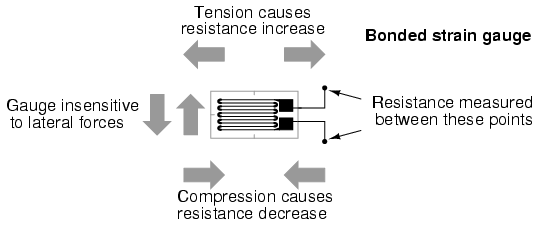
\includegraphics[width=\linewidth]{00204}
\centering
\caption{\label{strain} Schematic Diagram of a Strain Gauge, courtesy of National Instruments}
\end{figure}
\subsubsection{Apparatus Theory: Wheatstone Bridges}

Since strain measurements that are appropriate to measure with a strain gauge are typically on the order of millistrains, it is required to evaluate changes in resistance to high levels of accuracy; often as low as 0.1$\Omega$ \cite{wheatstone}. In order to measure such low changes, gauges are connected to the measurement system using a bridge configuration, and exploit a voltage excitation source. Typically, four resistors are used to construct the bridge, with an excitation voltage $V_{Ex}$ applied across it:
\begin{figure}[H]
\begin{center}


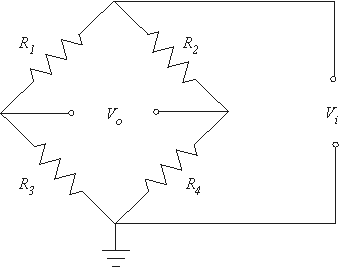
\includegraphics[width=.5\linewidth]{Graphic1}
\caption{\label{wheat}Schematic of a Wheatstone Bridge, courtesy of National Instruments}
\end{center}
\end{figure}


For this circuit, $V_o$ can be expressed as follows:

\begin{equation} \label{wheatstoneeq}
V_o = \bigg \lbrace \frac{R_3}{R_3 + R_4} - \frac{R_2}{R_1 + R_2} \bigg \rbrace \times V_i
\end{equation}

Clearly, from this equation, if:

\begin{equation}
\frac{R_1}{R_2} = \frac{R_4}{R_3}
\end{equation}

then the output $V_o$ is 0. Here, the bridge is said to be balanced. However, by replacing \textnormal{$R_4$} with a strain gauge of variable resistance, the bridge will become unbalanced and result in a non-zero output voltage. If it is to be assumed that \textnormal{$R_1 = R_2 = R_3$}, then it is possible to use equation \ref{gf} and \ref{wheatstoneeq} to give the ratio of output to input voltages in terms of strain:

\begin{equation}\label{bigdaddy}
\frac{V_o}{V_{Ex}} = -\frac{GF\times \varepsilon}{4} \bigg \lbrace \frac{1}{1 + GF\times \frac{\varepsilon}{2}} \bigg \rbrace
\end{equation}

Using equation \ref{bigdaddy}, it is trivial to calculate the strain on an object by simple measurement of the ratio of output voltage to input voltage if the gauge factor is known.


% GENERATE TABLE OF CONTENTS AND/OR TABLE OF FIGURES
% These seem to have some issues with the "revtex4" document class.  To use, change
% the very first line of this document to "article" like this:
% \documentclass[aps,letterpaper,10pt]{article}
%\tableofcontents
%\listoffigures
%\listoftables

\subsection{Method}\label{method}

\begin{enumerate}
\item The strain gauge amplifier should be warmed up and set to the correct gauge factor of 2.1.
\item Select gauge 1 and balance the bridge with the beam unloaded. Then, rotate the lever to bend the beam and note the strain gauge reading. Rotate the lever back to its original position.
\item Repeat step 2 for gauges 2 and 3 and note the strain.
\item Repeat step 2 for gauges 4 and 5, noting the strain in a second table.
\end{enumerate}

\section{Results}
\subsection{Measurements}
Following the experimental procedure outlined in \ref{method}, the following results were obtained, with all results in microstrain ($\mu$strain):

\begin{figure}[hb]
\begin{center}
\begin{tabular}{l | c | c | r}

 & \textbf{Gauge 1} & \textbf{Gauge 2} & \textbf{Gauge 3} \\
 \textbf{Unloaded} & 0 & 0 & 0 \\
 \textbf{Loaded} & 953 & 407 & -235 \\

\end{tabular}
\end{center}
\caption{\label{results1} Experimental results for strain gauges 1-3}
\end{figure}

\begin{figure}[ht]
\begin{center}
\begin{tabular}{l | c | r}

 & \textbf{Gauge 1} & \textbf{Gauge 2} \\
 \textbf{Unloaded} & 0 & 0  \\
 \textbf{Loaded} & -374 & 977 \\

\end{tabular}
\end{center}
\caption{\label{results2} Experimental results for strain gauges 4 and 5}
\end{figure}


\subsection{Analysis}

\emph{Mohr's circle analysis to go here.}

\section{Theoretical Predictions}

For the rectangular beam cross-section, the second moment of area is given by the following:

\begin{equation}
I = \frac{bd^3}{12} = \frac{25.4 \times 6.35^3}{12} = 542mm^4 = 5.42\times 10^{-10} m^4
\end{equation}

The tip deflection of a cantilever beam subject to a force F at the free end is \cite{mechengmat}:
\begin{equation}
\Delta = \frac{FL^3}{3EI}
\end{equation}
Assuming a Young's modulus for aluminium of E = $70\times 10^9 Nm^{-2}$ the required force to produce a deflection of 12.5mm is given by:

\begin{equation}
F = \frac{3EIV}{L^3} = \frac{3 \cdot 70 \times 10^9  \cdot 5.42 \times 10^{-10} \cdot 12.5 \times 10^{-3}}{0.254^3} = 86.82N
\end{equation}

\begin{figure}[ht]
\begin{center}


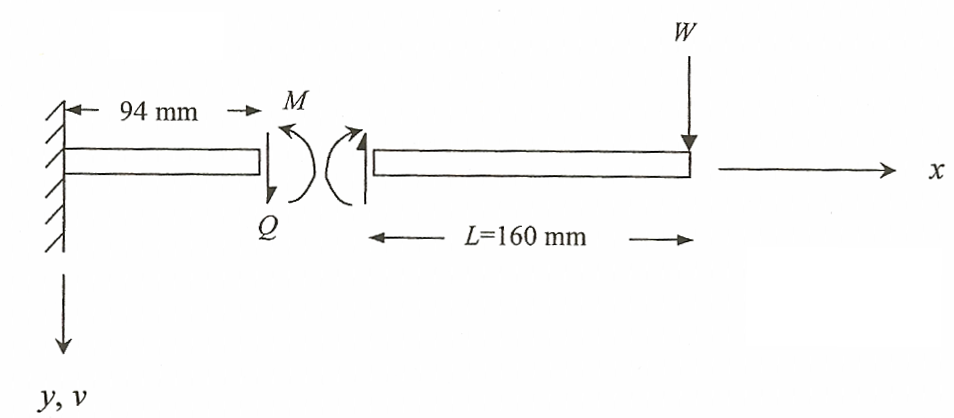
\includegraphics[width=\linewidth]{bending}
\caption{\label{bending}Bending moment at strain gauge location}
\end{center}
\end{figure}

At the strain gauge location, as shown in Figure \ref{bending}, the bending moment M is:

\begin{equation}
M = -F \cdot 0.16 = -13.89 Nm
\end{equation}

Now employing the expression $\sigma_{xx} = \frac{My}{I}$ \cite{bendingtheory}, with $y = -\frac{6.32}{2}mm = 3.175\times 10^{-3}$m for the upper beam surface, to give:

\begin{equation}
\sigma_{xx} = \frac{-13.89 \cdot -3.175\times 10^{-3}}{5.42\times 10^{-10}} = 81.36\times 10^6 \textnormal{ Nm}^{-2} = 81.4\textnormal{MPa}
\end{equation}

There is zero stress in the y- and z-directions, so Hooke's law reduces to:

\begin{equation}
\varepsilon = \frac{\sigma_{xx}}{E}, \varepsilon_{yy} = \varepsilon_{zz} = - \nu \varepsilon
\end{equation}

Thus

\begin{equation}
\varepsilon_{xx} = \frac{81.4\times 10^6}{70\times 10^9} = 1163\times 10^{-6} = 1163\mu \varepsilon, \varepsilon_{yy} = \varepsilon_{zz} = -0.3 \cdot 1163 = -349 \mu \varepsilon
\end{equation}

\section{Discussion}

There are clearly some discrepancies between the experimental results and the values predicted by theory. Perhaps most significant in 

\emph{Critical evaluation: Discuss, compare and evaluate the results in detail, comment on the potential sources of experimental error and the causes of any differences between the two sets of measurements, as well as any discrepancies  between experimental measurements and the theoretical predictions (also see the analysis section for aspects to be included here). 12 marks}
\section{Conclusion}
\emph{Sum up the main findings and conclusions of the study, including any experimental limitations.
…
[6 MARKS]
}
\newpage

\bibliographystyle{unsrt}
\bibliography{biblist}

\section{Nomenclature}
\begin{tabular}{l l}
\emph{b} & Breadth \\
\emph{d} & Depth \\
\emph{E} & Young's Modulus \\
\emph{I} & Second Moment of Area \\
\emph{L} & Length \\
\emph{M} & Bending Moment \\
\emph{F} & Load \\
\emph{x, y, z} & Cartesian Coordinates \\
\emph{$\varepsilon$} & Direct Strain \\
\emph{$\sigma$} & Direct Stress \\
\emph{$\Delta$} & Deflection \\


\end{tabular}

\end{document}